\chapter{Planning Your Observations And Travel}\label{chap:travel}

%++++++++++++++++++++++++++++++++++++++++++++++++++++++++++++++++++++++++++++
\section{Preparing for Your Observations}

After your proposal has been accepted you will be notified of how much
observing time you will receive on the \gls{GBT}.  You will also be notified
of who will be your scientific contact person (friend).  You should contact your
scientific support person well in advance of your observations to help you develop
observing strategies and your \glspl{SB}.

We require that new observers (or experienced observers doing new projects outside
their previous realm of experience) come to Green Bank for their initial observations.
Advisers are also required to accompany their students for their first trip to
Green Bank.

\begin{itemize}[leftmargin=*]
\item All policies are found at
\htmladdnormallink
{https://safe.nrao.edu/wiki/bin/view/GB/Observing/GbtObservingPolicies}
{https://safe.nrao.edu/wiki/bin/view/GB/Observing/GbtObservingPolicies}.
\item Room reservations can be made at
\htmladdnormallink
{https://bos.nrao.edu/reservations}
{https://bos.nrao.edu/reservations}.
\item Call +1 (304)-456-2227 for further information on reservations
and planning your travel.
\end{itemize}

Contact your GBT friend well in advance of the observations to determine the
optimum dates for your visit and ensure that the telescope and hardware
will be available for the project.

You should plan on being in Green Bank at least one full business day before
your observations begin.  This will allow you to meet with your scientific
support person as well as the staff support person who will be on-call
during your observations.

If your observations are dynamically scheduled and dependent on weather
conditions, you should plan to spend at least a week, and preferably two
weeks, to increase the likelihood that appropriate conditions for the 
observations will occur during your visit.


%++++++++++++++++++++++++++++++++++++++++++++++++++++++++++++++++++++++++++++
\section{Travel Support}

Some travel support for observing and data reduction is available for U.S. 
investigators on successful proposals. More information on the travel 
support that \gls{NRAO} provides can be found at \\
\htmladdnormallink{http://www.nrao.edu/admin/do/nonemployee\_observing\_travel.shtml}{http://www.nrao.edu/admin/do/nonemployee_observing_travel.shtml}.

%++++++++++++++++++++++++++++++++++++++++++++++++++++++++++++++++++++++++++++
\section{Trains, Planes and Automobiles}

In principle, observers may use a number of area airports for their travel to 
Green Bank.  These include Washington Dulles, Pittsburgh, Charlottesville, 
Roanoke (VA), Charleston (WV), Clarksburg (WV) or Lewisburg (WV). 
In addition, limited AMTRACK train service is available to Charlottesville 
and White Sulphur Springs, WV.  Rental cars are available at most of the 
airports.  If you do not have your own transportation, the Observatory can
also send a driver for pickup at any of these airports or stations.

%++++++++++++++++++++++++++++++++++++++++++++++++++++++++++++++++++++++++++++
\section{Housing}

The residence hall is available for astronomers while observing or reducing data
after completion of their observations. Single rooms (2 beds) are available for
\$55.00 (+tax) a day single occupancy or \$69.00 (+tax) per day per room double
occupancy. Students attending a degree conferring college or university and
coming to Green Bank to use the telescope will pay single room rate \$47.00
(+tax) or \$59.00 (+tax) per day double occupancy. In addition,
there are four one-bedroom apartments with equipped kitchens at \$83.00
(+tax) per day. Cribs, high chairs, and fold-up beds are also available. 
Costs of lodging at observatory facilities can be waived on request in advance
and on approval of the Site Director.


%++++++++++++++++++++++++++++++++++++++++++++++++++++++++++++++++++++++++++++
\section{Getting To Green Bank}


\subsection{Where is Green Bank?}

\begin{figure}
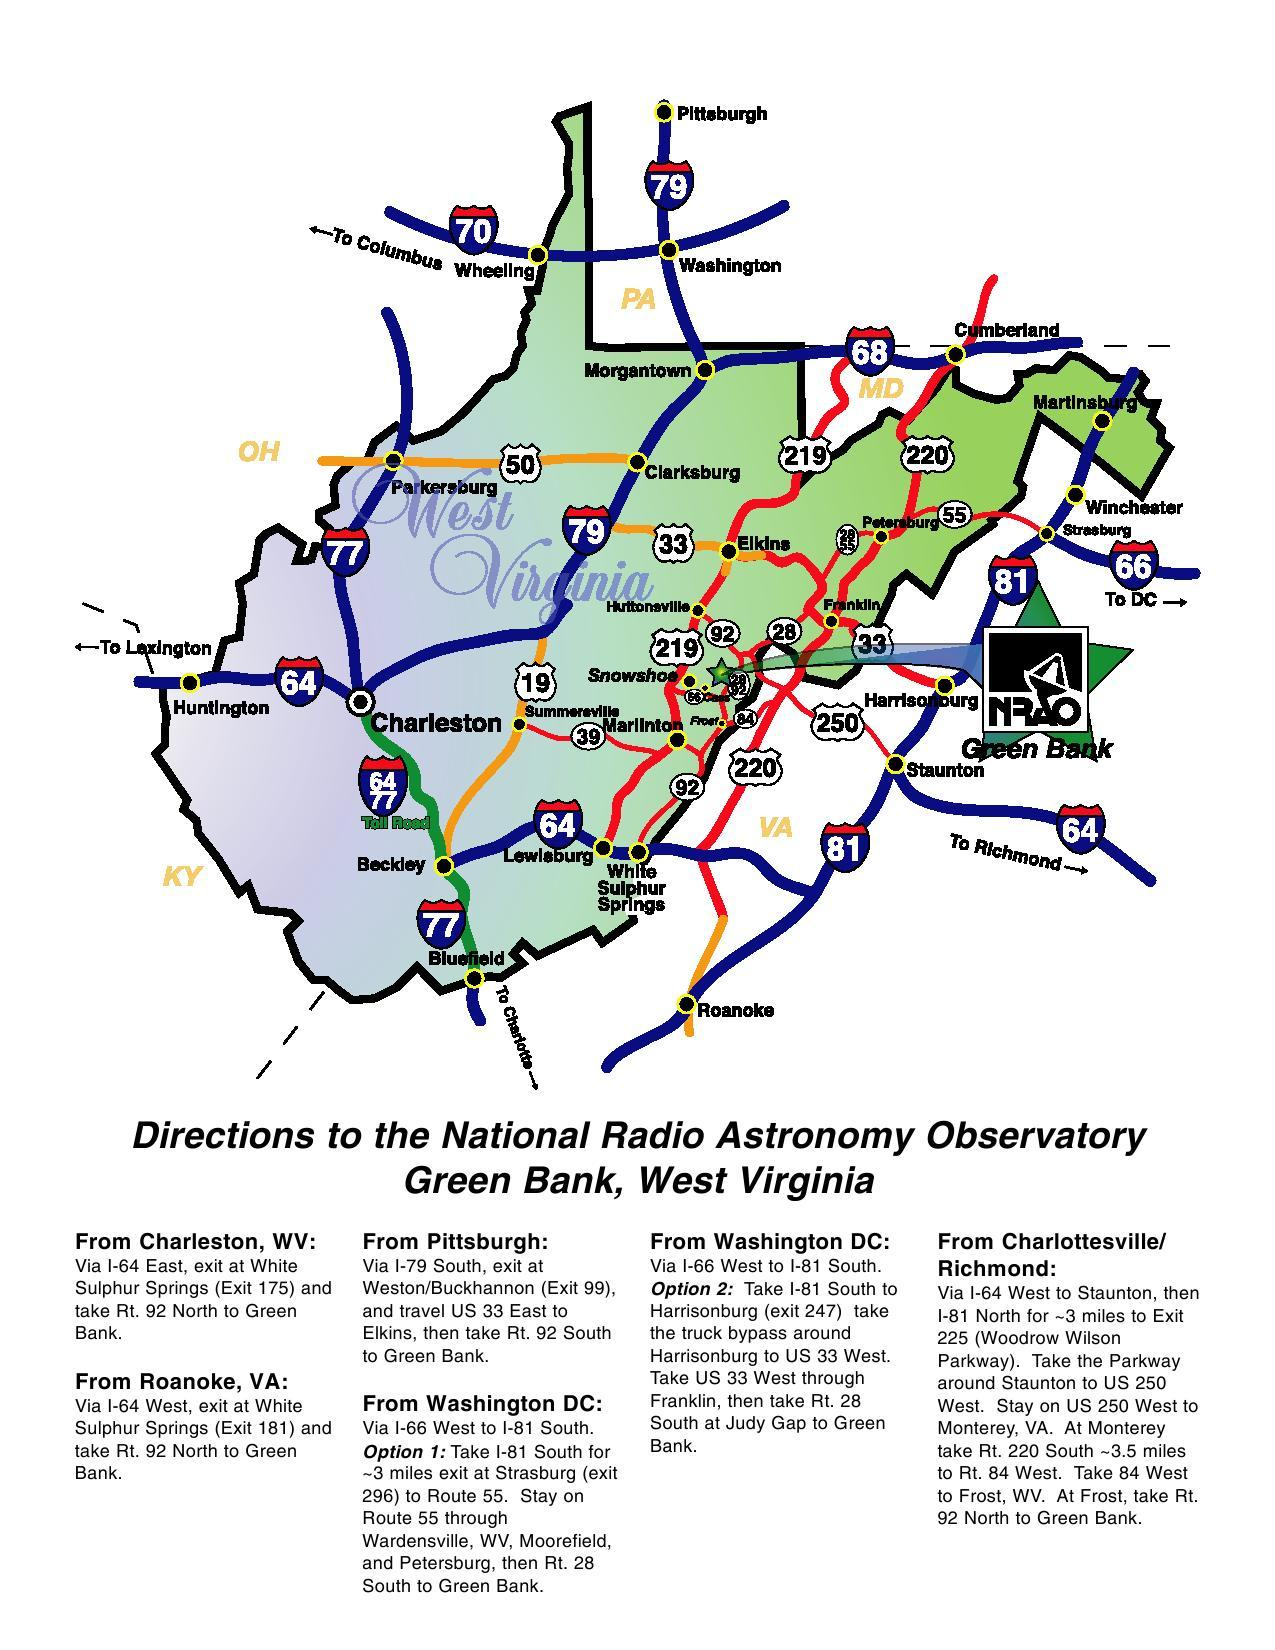
\includegraphics[width=7.0in,bb=0 0 1275 1650]{gbdirections.jpg}
\caption[Directions to Green Bank]{Direction to Green Bank.
\label{fig:directions}
}
\end{figure}

A map showing the location of Green Bank relative to major, nearby
towns and cities is shown in Figure~\ref{fig:directions}.  Simplified
directions are also shown in Figure~\ref{fig:directions}.

Green Bank is located in Pocahontas County, WV, very close to the Virginia
border and at about the mid-point of the full extent of the Virginia--West
Virginia border.


\subsection{Directions to Green Bank}

  The following are directions to Green Bank from airports in 
Pittsburgh, Pa, Washington, DC, Charlottesville, Va and Roanoke, Va. The 
duration of the drive from either Pittsburgh or Washington is 
four to five hours. The duration of the drive from Charlottesville 
and Roanoke is about 2--1/2 hours.

\subsubsection{Beware of GPS!!}

GPS systems, Mapquest, and other such automated route finding systems
are notoriously unreliable within 50 miles of the Observatory.
Some roads that are recommended by these systems are passable only with
4-wheel drive vehicles.
Do not turn onto unpaved roads !


\subsubsection{Pittsburgh to Green Bank}

From the Greater Pittsburgh International Airport, go east
   on route 60 to US 22/30. Follow 22/30 east to Interstate 79. 
   Take I-79 south through Clarksburg, WV to the US 33 exit (exit 99) near 
   Buckhannon, WV. Go east on US 33 through Buckhannon to Elkins, 
   WV. Turn south on US 250/219 to go to Huttonsville. In 
   Huttonsville, take US 250 (route 92) southeast to Bartow. 
   Follow route 92/28 south to Green Bank.

\subsubsection{Washington Dulles or National to Green Bank}

From the Washington Dulles International Airport, go south
   on route 28 to Interstate 66. 

From the Washington National Airport, take US 1/Va 110/US 50 to Interstate
66 (ask at airport for exact details).

Take I-66 west to I-81. From 
   here follow I-81 south to the exit for route 55 near 
   Strasburg, VA. Go west on 55 to Moorefield, WV. Turn 
   south on US 220/55, and drive to Petersburg, WV. Go 
   south on route 28/55 to Seneca Rocks. Continue south 
   on 28 through Judy Gap to Bartow. Follow route 92/28 
   south to Green Bank.

\subsubsection{Charlottesville to Green Bank}

From the Charlottesville-Albemarle Airport, go east (straight) 
   on Airport Road to US 29. Take 29 south to US 250, and follow 
   250 west to Interstate 64. Go west on I-64 to Interstate 81 
   near Staunton, VA. After traveling north on I-81 for about
   two miles, take the Woodrow Wilson Parkway exit. Go west on 
   the parkway to US 250, and follow 250 west to Monterey, VA. 
   In Monterey, turn south on US 220, and shortly thereafter,
   veer west on route 84 to go to Frost, WV. Follow route 
   92/28 north to Green Bank.

\subsubsection{Roanoke to Green Bank}

From the Roanoke Airport go left (south) on Valley View Drive/Airport
road and then almost immediately turn right onto Hershberger
Road.  Go about 1/2 mile and then take I-581 north to I-81
north.  Go two exits on I-81 north to US 220, the Daleville/Troutville
exit.  Take US 200 north toward (and through) Fincastle until
you reach I-64.  Take I-64 west to White Sulpher Springs, WV.
Take the first White Sulpher Springs exit and turn right.  After
about 1/2 mile turn right onto route 92 north and this will take
you to Green Bank.

\subsection{Once You Are in Green Bank}

The entrance to the observatory is about one-half mile north
of \dq{downtown} Green Bank on the west side of route 92/28
(see Figure~\ref{fig:sitemap}).
Look for the Jansky and Reber antennas. They are located on 
either side of the entrance.
\begin{figure}
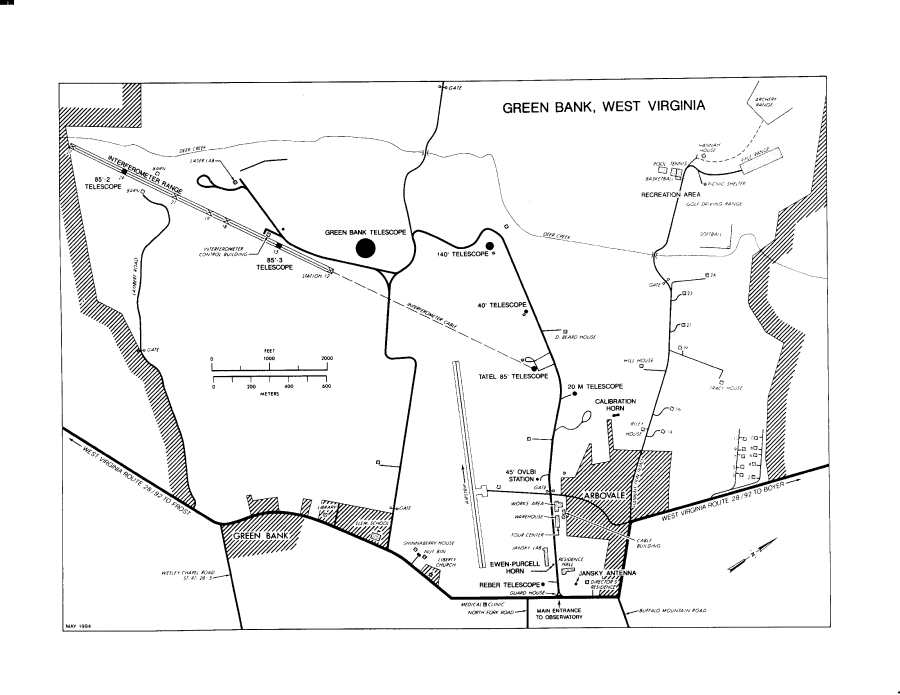
\includegraphics[width=6.0in,bb=0 0 900 695]{gbsitemap.jpg}
\caption[Green Bank Site Map]{NRAO, Green Bank site map.
\label{fig:sitemap}
}
\end{figure}
  
To pick up your room keys and site keycards you will need to come to the
Jansky Lab. The Jansky lab is the second building on the left as you
enter the site.  Go in the \dq{atrium} main entrance.  If after working
hours, use the telephone on the left to call the GBT operator at 2341.
The operator will then \dq{buzz you in}.  If during normal working hours,
just walk in. The room packets and keys will be found near the beginning
of the hallway on your right as you enter the Jansky Lab.

The residence hall is the first building on the right as one enters the
observatory. Adequate parking is provided on the west side of the residence
hall. Enter the residence hall through the double glass doors on the west
side of the building.  The observer's lounge is located on the second floor
of the residence hall, directly above the entrance.

